\documentclass{beamer}

\usepackage{tikz}
\usetikzlibrary{arrows}
\usepackage{hyperref}
\usepackage{fancyvrb}

\newcommand{\rnode}[1]{#1}
\newcommand{\nccurve}[1]{#1}

\newcommand{\bframe}[1]{\begin{frame}[fragile]{#1}}

\newcommand{\dt}{\Delta t}


\newcommand{\axes}{
  \draw[->,thick] (-1,0) -- (10,0);
  \draw[->,thick] (0,-1) -- (0,6);
}

\newcommand{\flowlines}{
  \draw[blue] (0,1) .. controls(4,4.5) .. (10,4.75);
  \draw[blue] (0,0) .. controls(4,4) .. (10,2.2);
  \draw[blue] (1,0) .. controls(4.5,3.125) .. (10,1);
  \draw[blue] (1.5,0) .. controls(4.5,2.7) .. (10,.5);
}

\newcommand{\point}[2]{
  %  \draw[fill=gray!30] (#1) circle (0.1) node[above] {\ensuremath{#2}}
  \node[circle, fill=blue] (#2) at (#1) {} ;
  \node[above] (foo) at (#1) {\ensuremath{#2}}
}

\newcommand{\points}{
  \point{1,1}{x_0};
  \point{4.4,3.3}{x_1};
  \point{9,2.5}{x_2};
}

\AtBeginSection[]
{
\bframe{Outline}
\tableofcontents[currentsection]
\end{frame}
}

\title{Game Physics Notes 02}
\author{CSCI 321}
\institute{WWU}

\begin{document}\small


\bframe{~}
\titlepage
\end{frame}

\bframe{Forces}

Newton's second law of motion: $F=ma$

\begin{eqnarray*}
a &=& F/m\\
v' &=& a\\
x' &=& v
\end{eqnarray*}
\begin{quotation}
Corpus omne perseverare in statu suo quiescendi vel movendi
uniformiter in directum, nisi quatenus a viribus impressis cogitur
statum illum mutare. 
\end{quotation}
Or, in English:
\begin{quotation}
Every body perseveres in its state of being at
rest or of moving uniformly straight forward, except insofar as it is
compelled to change its state by force impressed.
\end{quotation}
\end{frame}


\bframe{Forces and Motion}

\begin{eqnarray*}
F &=& ma\\
a &=& F/m\\
v' &=& a\\
x' &=& v
\end{eqnarray*}

\begin{itemize}
\item What we really want to know is: ``How do things move?''\pause
\item If we know the forces and masses, we know the acceleration.\pause
\item If we can integrate the acceleration we can get the velocity.\pause
\item If we can integrate the velocity we can get the position.\pause
\item The problem is integration---generally unsolvable.
\item So we use approximate integration.
\end{itemize}
\end{frame}

\bframe{The problem of Integration}

There exists a vector field, and exact integration of this field would
move a point along the flow lines.  But exact integration is
impossible in a discrete simulation.

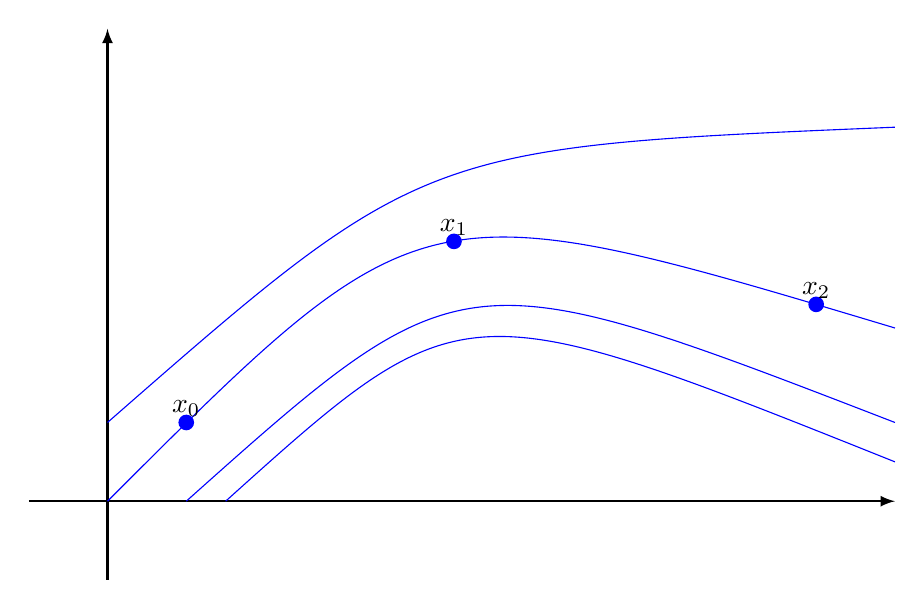
\begin{tikzpicture}[>=latex,every node/.style={inner sep=2pt}]
  \axes
  \flowlines
  \points
\end{tikzpicture}

\end{frame}

\bframe{Euler Integration}

We need to find the position for a given moment in time.  So we regard
position as a function of time, $x(t)$.  Assuming we know the position
at a given time, and we can also somehow figure out the velocity at
that time, $v(t)$, we find $x(t+\dt)$ by simply scaling the
velocity and adding it to the position.


\begin{eqnarray*}
{k(t)} &=& v(t)\Delta t\\
x(t+\dt) &=& x(t) + k
\end{eqnarray*}

For convenience we often write the sequence of points
\[
x(t), x(t+\dt), x(t+2\dt), \ldots
\]
as
\[
x_0, x_1, x_2, \ldots
\]

A similar operation can be used to update velocity, given acceleration.

\end{frame}
\bframe{Euler Integration}

\begin{eqnarray*}
a &=& F/m\\
v' &=& a\\
x' &=& v
\end{eqnarray*}

\bigskip


\begin{verbatim}
def update(x, v, F, m, dt):
  a = F(x, v) / m
  x += v * dt
  v += a * dt
\end{verbatim}

\bigskip
\begin{itemize}
  \item
Why do we update the position before the velocity?
\item
Run {\tt spring.py}
\end{itemize}
\end{frame}

\bframe{Euler Integration}

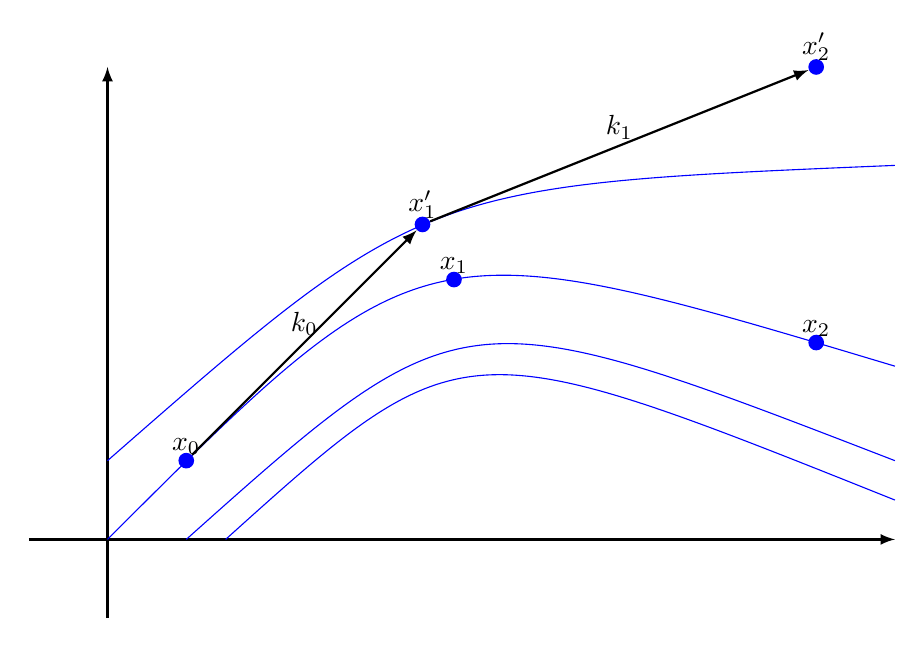
\begin{tikzpicture}[>=latex,every node/.style={inner sep=2pt}]
  \axes
  \flowlines
  \points
  % vectors for euler
  \point{4,4}{x_1'};
  \point{9,6}{x_2'};
  \draw[thick,->] (x_0) -- node[above] {$k_0$}  (x_1');
  \draw[thick,->] (x_1') -- node[above] {$k_1$} (x_2');
\end{tikzpicture}

\end{frame}



\bframe{Euler Calculations, $\dt= 1$}

\begin{minipage}{2in}
\begin{eqnarray*}
m &=& 10  \\
k &=& 5   \\
f &=& -kx \\
x' &=& v \\
v' &=& a \\
a &\leftarrow& f/m = -kx/m = -x/2 \\
x &\leftarrow& x +  x'\dt = x +  v \dt \\
v &\leftarrow& v +  v'\dt = v +  a \dt \\
\end{eqnarray*}
\end{minipage}
\hfill\begin{minipage}{2in}


\begin{tabular}{r|rrrr}
$t$ & $x$ & $v$ & $a$ \\\hline
0.0  &  20.0  &  0.0  &  -10.0  &  \\
1.0  &  20.0  &  -10.0  &  -10.0  &  \\
2.0  &  10.0  &  -20.0  &  -5.0  &  \\
3.0  &  -10.0  &  -25.0  &  5.0  &  \\
4.0  &  -35.0  &  -20.0  &  17.5  &  \\
5.0  &  -55.0  &  -2.5  &  27.5  &  \\
\end{tabular}


\end{minipage}


\end{frame}

\bframe{Euler Calculations, $\dt= 0.5$}

\begin{minipage}{2in}
\begin{eqnarray*}
m &=& 10  \\
k &=& 5   \\
f &=& -kx \\
x' &=& v \\
v' &=& a \\
a &\leftarrow& f/m = -kx/m = -x/2 \\
x &\leftarrow& x + x'\dt = x + v\dt \\
v &\leftarrow& v + v' = v\dt + a\dt \\
\end{eqnarray*}
\end{minipage}
\hfill\begin{minipage}{2in}

\begin{tabular}{r|rrrr}
$t$ & $x$ & $v$ & $a$ \\\hline
0.0  &  20.0  &  0.0  &  -10.0  &  \\
0.5  &  20.0  &  -5.0  &  -10.0  &  \\
1.0  &  17.5  &  -10.0  &  -8.8  &  \\
1.5  &  12.5  &  -14.4  &  -6.3  &  \\
2.0  &  5.3  &  -17.5  &  -2.7  &  \\
2.5  &  -3.4  &  -18.8  &  1.7  &  \\
3.0  &  -12.9  &  -18.0  &  6.4  &  \\
3.5  &  -21.8  &  -14.8  &  10.9  &  \\
4.0  &  -29.2  &  -9.3  &  14.6  &  \\
4.5  &  -33.9  &  -2.0  &  16.9  &  \\
5.0  &  -34.9  &  6.5  &  17.4  &  \\
\end{tabular}
\end{minipage}


\end{frame}

\bframe{Euler Calculations, $\dt = 0.25$}

\begin{minipage}{2in}
\begin{eqnarray*}
m &=& 10  \\
k &=& 5   \\
f &=& -kx \\
x' &=& v \\
v' &=& a \\
a &\leftarrow& f/m = -kx/m = -x/2 \\
x &\leftarrow& x + x'\dt = x + v \dt\\
v &\leftarrow& v + v'\dt = v + a \dt\\
\end{eqnarray*}
\end{minipage}
\hfill\begin{minipage}{2in}



{\scriptsize
\begin{tabular}{r|rrrr}
$t$ & $x$ & $v$ & $a$ \\\hline
0.0  &  20.0  &  0.0  &  -10.0  &  \\
0.3  &  20.0  &  -2.5  &  -10.0  &  \\
0.5  &  19.4  &  -5.0  &  -9.7  &  \\
0.8  &  18.1  &  -7.4  &  -9.1  &  \\
1.0  &  16.3  &  -9.7  &  -8.1  &  \\
1.3  &  13.8  &  -11.7  &  -6.9  &  \\
1.5  &  10.9  &  -13.5  &  -5.5  &  \\
1.8  &  7.6  &  -14.8  &  -3.8  &  \\
2.0  &  3.9  &  -15.8  &  -1.9  &  \\
2.3  &  -0.1  &  -16.2  &  0.0  &  \\
2.5  &  -4.2  &  -16.2  &  2.1  &  \\
2.8  &  -8.2  &  -15.7  &  4.1  &  \\
3.0  &  -12.1  &  -14.7  &  6.1  &  \\
3.3  &  -15.8  &  -13.2  &  7.9  &  \\
3.5  &  -19.1  &  -11.2  &  9.6  &  \\
3.8  &  -21.9  &  -8.8  &  10.9  &  \\
4.0  &  -24.1  &  -6.1  &  12.1  &  \\
4.3  &  -25.6  &  -3.1  &  12.8  &  \\
4.5  &  -26.4  &  0.1  &  13.2  &  \\
4.8  &  -26.3  &  3.4  &  13.2  &  \\
5.0  &  -25.5  &  6.7  &  12.7  &  \\
\end{tabular}
}



\end{minipage}

\end{frame}


\bframe{Online discussions of Midpoint and Runge Kutta}

Readings:
\begin{itemize}
\item \url{http://www.pixar.com/companyinfo/research/pbm2001/},
  Differential equation basics, and Particle dynamics
\item \url{http://www.nrbook.com/c/}, 16.0, 16.1
\end{itemize}
\end{frame}

\bframe{Midpoint Method}

\begin{eqnarray*}
  {k}_1 &=&  v\Delta t\\
  x_{half} &=& x + k_1/2\\
{k}_2 &=& v_{half}\Delta t \\
{x} &\leftarrow& {x} + {k}_2 
\end{eqnarray*}

\begin{itemize}
\item
Euler method has errors $O(\Delta t^2)$
\item
Midpoint method has errors $O(\Delta t^3)$
\item Can take steps twice as big and get smaller errors:
\begin{eqnarray*}
0.05^2 &=& 0.0025\\
0.10^3 &=& 0.001
\end{eqnarray*}
\end{itemize}
\end{frame}

\bframe{Midpoint Method} Move point halfway along vector.

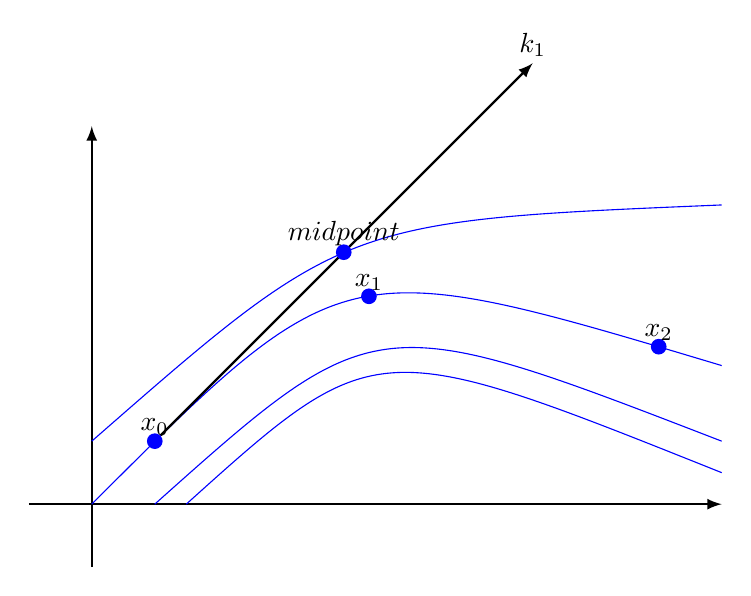
\begin{tikzpicture}[>=latex,scale=0.8,every node/.style={inner sep=2pt}]
  \axes
  \flowlines
  \points
  % First Midpoint vector
  \draw[thick,->] (x_0) -- (7,7) node[above] {$k_1$};
  \point{4,4}{midpoint};
\end{tikzpicture}

\end{frame}

\bframe{Midpoint Method} Find new derivative at halfway point.

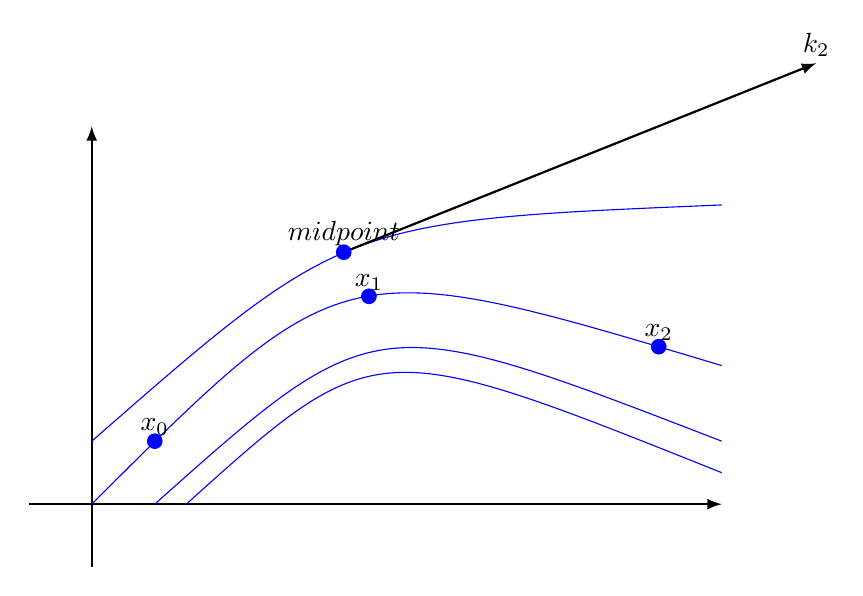
\begin{tikzpicture}[>=latex,scale=0.8,every node/.style={inner sep=2pt}]
  \axes
  \flowlines
  \points
  % Second Midpoint vector
  \draw[thick,->] (4,4) -- (11.5,7) node[above] {$k_2$};
  \point{4,4}{midpoint};
\end{tikzpicture}

\end{frame}

\bframe{Midpoint Method} Translate new vector back to start.

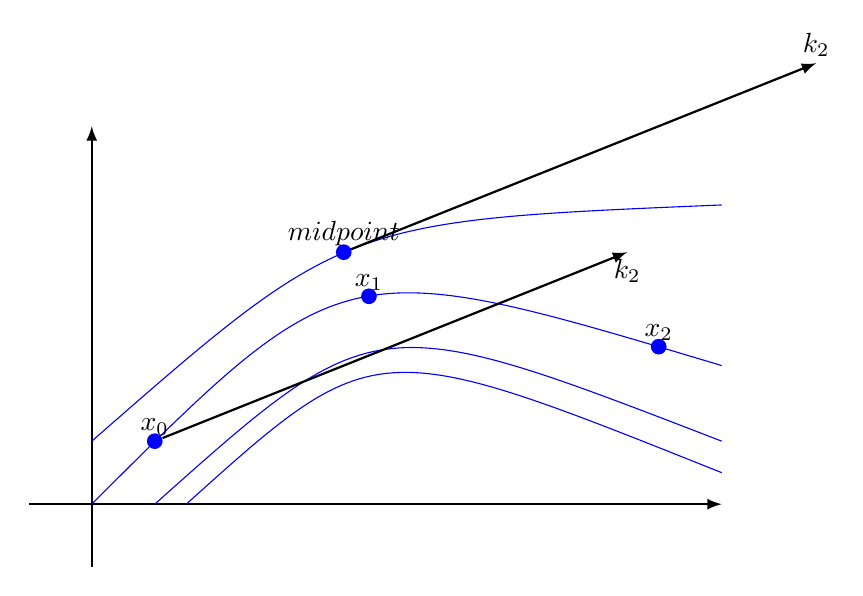
\begin{tikzpicture}[>=latex,scale=0.8,every node/.style={inner sep=2pt}]
  \axes
  \flowlines
  \points
  % Translate Midpoint vector
  \draw[thick,->] (4,4) -- (11.5,7) node[above] {$k_2$};
  \draw[thick,->] (x_0) -- (8.5,4) node[below] {$k_2$};
  \point{4,4}{midpoint};
\end{tikzpicture}

\end{frame}

\bframe{Midpoint Method} Add translated vector to start.

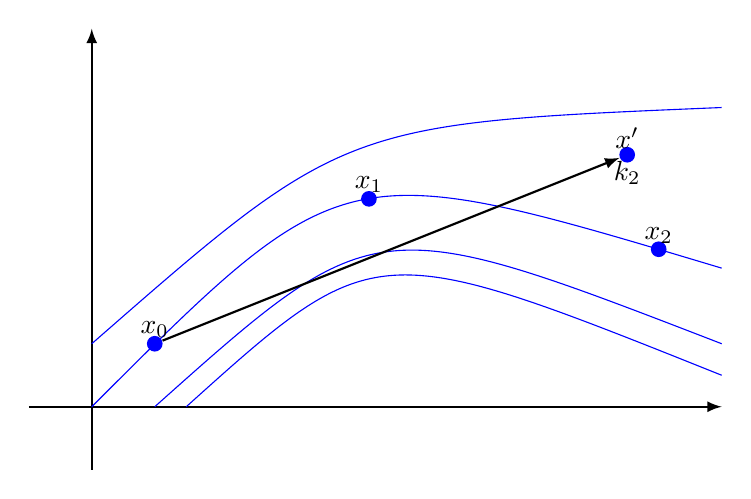
\begin{tikzpicture}[>=latex,scale=0.8,every node/.style={inner sep=2pt}]
  \axes
  \flowlines
  \points
  % Translate Midpoint vector
  \point{8.5,4}{x'};
  \draw[thick,->] (x_0) -- (x') node[below] {$k_2$};
\end{tikzpicture}

\end{frame}

\bframe{Midpoint Method} More accurate than Euler with same cost.

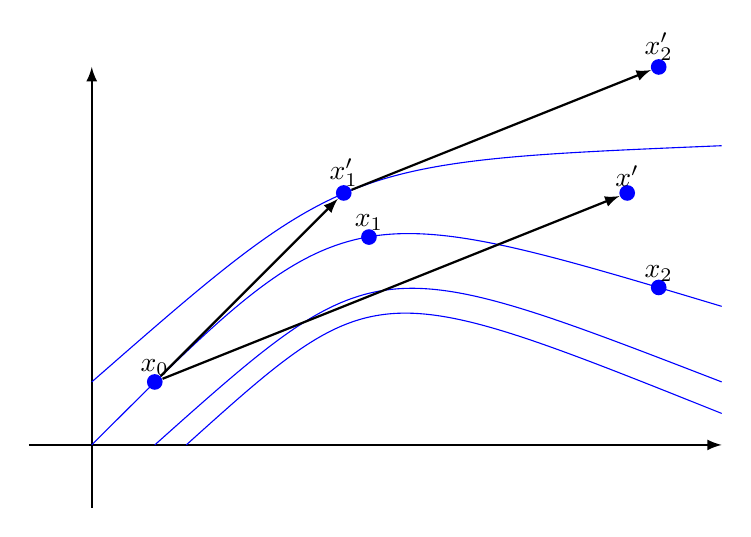
\begin{tikzpicture}[>=latex,scale=0.8,every node/.style={inner sep=2pt}]
  \axes
  \flowlines
  \points
  % Translate Midpoint vector
  \point{8.5,4}{x'};
  \draw[thick,->] (x_0) -- (x');
  % vectors for euler
  \point{4,4}{x_1'};
  \point{9,6}{x_2'};
  \draw[thick,->] (x_0) --  (x_1');
  \draw[thick,->] (x_1') -- (x_2');
\end{tikzpicture}

\end{frame}


\bframe{Midpoint Calculations, $\dt=2$}
\begin{minipage}{2in}
\begin{eqnarray*}
\dt &=& 2 \\
m &=& 10  \\
k &=& 5   \\
f &=& -kx \\
x' &=& v \\
v' &=& a \\
a &\leftarrow& f/m = -kx/m = -x/2 \\
v_{half} &\leftarrow& v + a\dt/2\\
x_{half} &\leftarrow& x + v\dt/2 \\
a_{half} &\leftarrow& -x_{half}/2 \\
v &\leftarrow& v + a_{half}\dt\\
x &\leftarrow& x + v_{half}\dt\\
\end{eqnarray*}
\end{minipage}\hfill
\begin{minipage}{2in}

\begin{tabular}{r|rrrr}
$t$ & $x$ & $v$ & $a$ \\\hline
0.0  &  20.0  &  0.0  &  -10.0  &  \\
1.0  &  20.0  &  -10.0  &  -10.0  &  \\
2.0  &  0.0  &  -20.0  &  -0.0  &  \\
3.0  &  -20.0  &  -20.0  &  10.0  &  \\
4.0  &  -40.0  &  0.0  &  20.0  &  \\
5.0  &  -40.0  &  20.0  &  20.0  &  \\
\end{tabular}

\end{minipage}

\hfill At $t=5$ Euler with $\dt=1$ had $x=-55$.

\end{frame}

\bframe{Midpoint Calculations, $\dt=1$}
\begin{minipage}{2in}
\begin{eqnarray*}
m &=& 10  \\
k &=& 5   \\
f &=& -kx \\
x' &=& v \\
v' &=& a \\
a &\leftarrow& f/m = -kx/m = -x/2 \\
v_{half} &\leftarrow& v + a\dt/2\\
x_{half} &\leftarrow& x + v\dt/2 \\
a_{half} &\leftarrow& -x_{half}/2 \\
v &\leftarrow& v + a_{half}\dt\\
x &\leftarrow& x + v_{half}\dt\\
\end{eqnarray*}
\end{minipage}\hfill
\begin{minipage}{2in}

\begin{tabular}{r|rrrr}
$t$ & $x$ & $v$ & $a$ \\\hline
0.0  &  20.0  &  0.0  &  -10.0  &  \\
0.5  &  20.0  &  -5.0  &  -10.0  &  \\
1.0  &  15.0  &  -10.0  &  -7.5  &  \\
1.5  &  10.0  &  -13.8  &  -5.0  &  \\
2.0  &  1.3  &  -15.0  &  -0.6  &  \\
2.5  &  -6.3  &  -15.3  &  3.1  &  \\
3.0  &  -14.1  &  -11.9  &  7.0  &  \\
3.5  &  -20.0  &  -8.4  &  10.0  &  \\
4.0  &  -22.4  &  -1.9  &  11.2  &  \\
4.5  &  -23.4  &  3.7  &  11.7  &  \\
5.0  &  -18.7  &  9.8  &  9.3  &  \\
5.5  &  -13.8  &  14.5  &  6.9  &  \\
\end{tabular}

\end{minipage}

\hfill At $t=5$ Euler with $\dt=0.5$ had $x=-34.9$.

\end{frame}

\bframe{Midpoint Calculations, $\dt=0.5$}
\begin{minipage}{2in}
\begin{eqnarray*}
m &=& 10  \\
k &=& 5   \\
f &=& -kx \\
x' &=& v \\
v' &=& a \\
a &\leftarrow& f/m = -kx/m = -x/2 \\
v_{half} &\leftarrow& v + a\dt/2\\
x_{half} &\leftarrow& x + v\dt/2 \\
a_{half} &\leftarrow& -x_{half}/2 \\
v &\leftarrow& v + a_{half}\dt\\
x &\leftarrow& x + v_{half}\dt\\
\end{eqnarray*}
\end{minipage}\hfill
\begin{minipage}{2in}

{\scriptsize
\begin{tabular}{r|rrrr}
$t$ & $x$ & $v$ & $a$ \\\hline
0.0  &  20.0  &  0.0  &  -10.0  &  \\
0.3  &  20.0  &  -2.5  &  -10.0  &  \\
0.5  &  18.8  &  -5.0  &  -9.4  &  \\
0.8  &  17.5  &  -7.3  &  -8.8  &  \\
1.0  &  15.1  &  -9.4  &  -7.5  &  \\
1.3  &  12.7  &  -11.3  &  -6.4  &  \\
1.5  &  9.4  &  -12.6  &  -4.7  &  \\
1.8  &  6.3  &  -13.7  &  -3.2  &  \\
2.0  &  2.6  &  -14.1  &  -1.3  &  \\
2.3  &  -1.0  &  -14.5  &  0.5  &  \\
2.5  &  -4.7  &  -13.9  &  2.3  &  \\
2.8  &  -8.1  &  -13.3  &  4.1  &  \\
3.0  &  -11.3  &  -11.9  &  5.7  &  \\
3.3  &  -14.3  &  -10.5  &  7.1  &  \\
3.5  &  -16.5  &  -8.3  &  8.3  &  \\
3.8  &  -18.6  &  -6.2  &  9.3  &  \\
4.0  &  -19.6  &  -3.6  &  9.8  &  \\
4.3  &  -20.6  &  -1.2  &  10.3  &  \\
4.5  &  -20.2  &  1.5  &  10.1  &  \\
4.8  &  -19.9  &  4.0  &  9.9  &  \\
5.0  &  -18.2  &  6.5  &  9.1  &  \\
5.3  &  -16.6  &  8.7  &  8.3  &  \\
\end{tabular}
}
\end{minipage}

\hfill At $t=5$ Euler with $\dt=0.25$ had $x=-25.5$.

\end{frame}


\bframe{ Fourth Order Runge-Kutta}
\begin{eqnarray*}
  k_1 &=& v\dt\\
  x_a &=& x + k_1/2\\
  k_2 &=& v_a\dt\\
  x_b &=& x + k_2/2\\
  k_3 &=& v_b\dt\\
  x_c &=& x+k_3\\
  k_4 &=& v_c\dt\\\\
  x &\leftarrow& x + \frac{k_1}{6} + \frac{k_2}{3} + \frac{k_3}{3} +
  \frac{k_4}{6} 
\end{eqnarray*}
\end{frame}

\bframe{Fourth order Runge Kutta}
Final vector used:
$\frac{{k}_1}{6}+\frac{{k}_2}{3}+\frac{{k}_3}{3}+\frac{{k}_4}{6}$


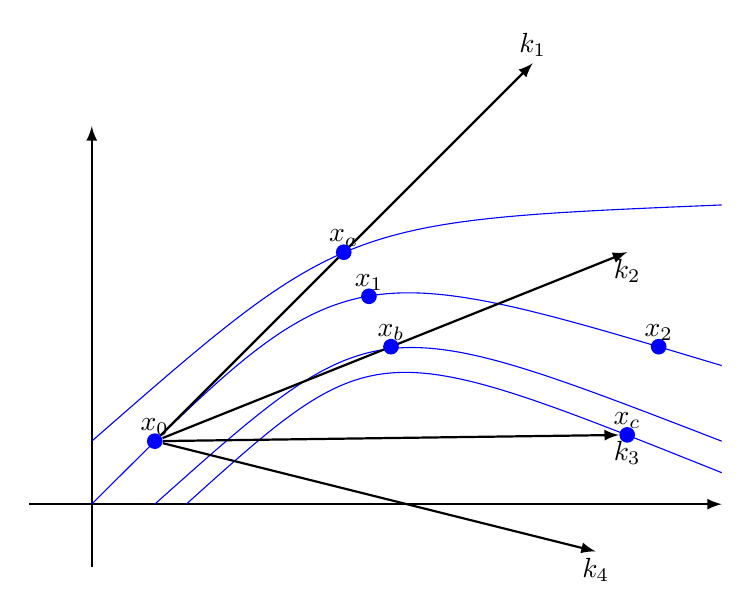
\begin{tikzpicture}[>=latex,scale=0.8,every node/.style={inner sep=2pt}]
  \axes
  \flowlines
  \points
  % First Midpoint vector
  \draw[thick,->] (x_0) -- (7,7) node[above] {$k_1$};
  \point{4,4}{x_a};
  \draw[thick,->] (x_0) -- (8.5,4) node[below] {$k_2$};
  \point{4.75,2.5}{x_b};
  \point{8.5,1.1}{x_c};
  \draw[thick,->] (x_0) -- (x_c) node[below] {$k_3$};
  \draw[thick,->] (x_0) -- (8,-0.75) node[below] {$k_4$};
\end{tikzpicture}


\end{frame}


\bframe{Fourth Order Runge Kutta Calculations, $\dt= 4$}

\begin{minipage}{2in}
\begin{eqnarray*}
m &=& 10  \\
k &=& 5   \\
f &=& -kx \\
x' &=& v \\
v' &=& a \\
a &\leftarrow& f/m = -kx/m = -x/2 \\
\end{eqnarray*}
\end{minipage}
\hfill\begin{minipage}{2in}

\begin{tabular}{r|rrrr}
$t$ & $x$ & $v$ & $a$ \\\hline
0.0  &  20.0  &  0.0  &  -10.0  &  \\
2.0  &  20.0  &  -20.0  &  -10.0  &  \\
2.0  &  -20.0  &  -20.0  &  10.0  &  \\
4.0  &  -60.0  &  40.0  &  30.0  &  \\
4.0  &  2.2  &  13.3  &  -1.1  &  \\
6.0  &  28.9  &  11.1  &  -14.4  &  \\
6.0  &  24.4  &  -15.6  &  -12.2  &  \\
8.0  &  -60.0  &  -35.6  &  30.0  &  \\
8.0  &  -29.4  &  -3.0  &  14.7  &  \\
10.0  &  -35.3  &  26.4  &  17.7  &  \\
10.0  &  23.5  &  32.3  &  -11.7  &  \\
12.0  &  100.0  &  -49.9  &  -50.0  &  \\
12.0  &  3.3  &  -18.6  &  -1.7  &  \\
\end{tabular}

\end{minipage}

\end{frame}



\bframe{Fourth Order Runge Kutta Calculations, $\dt= 2$}

\begin{minipage}{2in}
\begin{eqnarray*}
m &=& 10  \\
k &=& 5   \\
f &=& -kx \\
x' &=& v \\
v' &=& a \\
a &\leftarrow& f/m = -kx/m = -x/2 \\
\end{eqnarray*}
\end{minipage}
\hfill\begin{minipage}{2in}


\begin{tabular}{r|rrrr}
$t$ & $x$ & $v$ & $a$ \\\hline
0.0  &  20.0  &  0.0  &  -10.0  &  \\
1.0  &  20.0  &  -10.0  &  -10.0  &  \\
1.0  &  10.0  &  -10.0  &  -5.0  &  \\
2.0  &  0.0  &  -10.0  &  -0.0  &  \\
2.0  &  -1.1  &  -13.3  &  0.6  &  \\
3.0  &  -14.4  &  -12.8  &  7.2  &  \\
3.0  &  -13.9  &  -6.1  &  6.9  &  \\
4.0  &  -13.3  &  0.6  &  6.7  &  \\
4.0  &  -14.0  &  -1.5  &  7.0  &  \\
5.0  &  -15.5  &  5.5  &  7.7  &  \\
5.0  &  -8.5  &  6.3  &  4.2  &  \\
6.0  &  -1.5  &  7.0  &  0.7  &  \\
6.0  &  -0.8  &  9.1  &  0.4  &  \\
7.0  &  8.3  &  9.5  &  -4.2  &  \\
7.0  &  8.7  &  4.9  &  -4.4  &  \\
8.0  &  9.1  &  0.4  &  -4.5  &  \\
8.0  &  9.6  &  2.0  &  -4.8  &  \\
\end{tabular}

\end{minipage}

\end{frame}



\bframe{Fourth Order Runge Kutta Calculations, $\dt= 1$}

\begin{minipage}{2in}
\begin{eqnarray*}
m &=& 10  \\
k &=& 5   \\
f &=& -kx \\
x' &=& v \\
v' &=& a \\
a &\leftarrow& f/m = -kx/m = -x/2 \\
\end{eqnarray*}
\end{minipage}
\hfill\begin{minipage}{2in}
{\scriptsize
\begin{tabular}{r|rrrr}
$t$ & $x$ & $v$ & $a$ \\\hline
0.0  &  20.0  &  0.0  &  -10.0  &  \\
0.5  &  20.0  &  -5.0  &  -10.0  &  \\
0.5  &  17.5  &  -5.0  &  -8.8  &  \\
1.0  &  15.0  &  -8.8  &  -7.5  &  \\
1.0  &  13.7  &  -9.2  &  -6.8  &  \\
1.5  &  9.1  &  -12.6  &  -4.5  &  \\
1.5  &  7.4  &  -11.4  &  -3.7  &  \\
2.0  &  2.2  &  -12.9  &  -1.1  &  \\
2.0  &  1.3  &  -13.2  &  -0.7  &  \\
2.5  &  -5.3  &  -13.6  &  2.6  &  \\
2.5  &  -5.5  &  -11.9  &  2.7  &  \\
3.0  &  -10.6  &  -10.5  &  5.3  &  \\
3.0  &  -10.7  &  -10.7  &  5.4  &  \\
3.5  &  -16.0  &  -8.0  &  8.0  &  \\
3.5  &  -14.7  &  -6.7  &  7.4  &  \\
4.0  &  -17.4  &  -3.3  &  8.7  &  \\
4.0  &  -16.7  &  -3.2  &  8.3  &  \\
4.5  &  -18.3  &  1.0  &  9.1  &  \\
4.5  &  -16.2  &  1.4  &  8.1  &  \\
5.0  &  -15.3  &  4.9  &  7.7  &  \\
5.0  &  -14.2  &  5.2  &  7.1  &  \\
5.5  &  -11.6  &  8.8  &  5.8  &  \\
5.5  &  -9.8  &  8.1  &  4.9  &  \\
6.0  &  -6.1  &  10.1  &  3.1  &  \\
6.0  &  -5.2  &  10.5  &  2.6  &  \\
\end{tabular}
}
\end{minipage}

\end{frame}


\bframe{ Fourth Order Runge-Kutta}
\begin{itemize}
\item
Euler method has errors $O(\Delta t^2)$
\item
Midpoint method has errors $O(\Delta t^3)$
\item
Fourth order Runge Kutta has errors $O(\Delta t^5)$
\end{itemize}

\begin{eqnarray*}
0.05^2 &=& 0.00250\\
0.10^3 &=& 0.00100\\
0.20^5 &=& 0.00032
\end{eqnarray*}


\end{frame}

\bframe{Stepsize Matching Refresh Rate}
\begin{itemize}
\item The simplest approach to stepsize is to use the framerate:
  \begin{Verbatim}[frame=single]
framerate = 30.0
t = 0.0
dt = 1.0/framerate
while !quitting:
  clock.tick(framerate)
  handle.input()
  integrate(state, t, dt)
  t += dt
  display()
\end{Verbatim}

\item This may be OK for simple games, but if more accuracy is
  needed the physics should use as small a timestep as possible.
\item Also, the game refresh rate may not keep up with the nominal
  clock rate.
\end{itemize}
\end{frame}


\bframe{Stepsize Matching Refresh Rate $\times n$}
\begin{itemize}
\item Can also match $n$ steps to each frame:
  \begin{Verbatim}[frame=single]
framerate = 30.0
t = 0.0
dt = 1.0/framerate
while !quitting:
  clock.tick(framerate)
  handle.input()
  for i in range(n):
     integrate(state, t, dt/n)
  t += dt
  display()
\end{Verbatim}

\end{itemize}
\end{frame}

\bframe{Use actual timestep}
\begin{itemize}
\item {\tt clock.tick} returns milliseconds since last call.
  \begin{Verbatim}[frame=single]
framerate = 30.0
t = 0.0
while !quitting:
  dt = clock.tick(framerate) * 0.001
  handle.input()
  integrate(state, t, dt)
  t += dt       
  display()
  \end{Verbatim}
  \item Physics will be ``same'' regardless of computer's speed.
\item But again physics update should be as fast as possible
  for most realism.
  \item We could increase the framerate, but then we'd be doing
    unnecessary rendering.
\end{itemize}
\end{frame}

\bframe{Use smaller time step}
\begin{itemize}
  \begin{Verbatim}[frame=single]
framerate = 30.0
t = 0.0
dt = 0.01
while !quitting:
  timespan = clock.tick(framerate) * 0.001
  handle.input()
  while (timespan > 0):
    integrate(state, t, dt)
    timespan -= dt
  display()
\end{Verbatim}
\item Problem with the fractional part of {\tt dt}?
  \begin{itemize}  \item Can interpolate for fractional {\tt dt}.
    \end{itemize}
\item What if the physics gets behind?  Spiral of death!
  \begin{itemize}
  \item Make sure your physics can keep up with {\tt dt}.
    \end{itemize}
\end{itemize}
\end{frame}

\bframe{Use separate time for display and physics}
\begin{itemize}
  \begin{Verbatim}[frame=single]
framerate = 30.0
rendertime, physicstime = 0.0, 0.0
dt = 0.01
while !quitting:
  rendertime += clock.tick(framerate) * 0.001
  handle.input()
  while (physicstime < rendertime):
    integrate(state, physicstime, dt)
    physicstime += dt
  display()
\end{Verbatim}
\item Spiral of death still possible.
  \begin{itemize}
  \item Note: matching stepsize to framerate$\times n$ avoids death spiral.
  \end{itemize}
  
  \item Leftover fraction of {\tt dt} is carried forward to next
    render. 
  \item Can interpolate again for fractional {\tt dt}.
\item Note that {\tt dt} can be {\em longer} than time for a frame and it still
  works.
\end{itemize}
\end{frame}


\bframe{Differential Equations}
Reading:
\begin{itemize}
\item Strange attractors
\url{http://en.wikipedia.org/wiki/Attractor}

\item Run: {\tt strange??.py}

\item The Limits to Growth

{
\tiny

\setlength{\parindent}{-1cm}

%\url{http://www.csiro.au/files/files/plje.pdf}
\url{http://www.manicore.com/fichiers/Turner_Meadows_vs_historical_data.pdf}


%\url{http://www.csiro.au/files/files/plje.pdf}
\url{http://www.theguardian.com/commentisfree/2014/sep/02/limits-to-growth-was-right-new-research-shows-were-nearing-collapse}


}

\end{itemize}
\end{frame}

\bframe{Symplectic Euler/Semi-implicit Euler}
\begin{itemize}
\item \url{http://en.wikipedia.org/wiki/Semi-implicit_Euler_method}
\item Two forms:
\begin{eqnarray*}
v_{n+1} &=& v_{n} + a_{n}\Delta t\\
p_{n+1} &=& p_{n} + v_{n+1}\Delta t
\end{eqnarray*}
and
\begin{eqnarray*}
p_{n+1} &=& p_{n} + v_{n}\Delta t\\
v_{n+1} &=& v_{n} + a_{n+1}\Delta t
\end{eqnarray*}
\item Can use either one by itself, or alternate between them.
\item Not accurate, but almost conserves energy.
\item Easy to program when updates are by assignment.
\end{itemize}
\end{frame}

\bframe{Comparing Euler and Symplectic Euler, $\dt = 1$}

\begin{minipage}{0.45\textwidth}
{\scriptsize
  Euler
\begin{tabular}{r|rrrr}
$t$ & $x$ & $v$ & $a$ \\\hline
0.0  &  20.0  &  0.0  &  -10.0  &  \\
1.0  &  20.0  &  -10.0  &  -10.0  &  \\
2.0  &  10.0  &  -20.0  &  -5.0  &  \\
3.0  &  -10.0  &  -25.0  &  5.0  &  \\
4.0  &  -35.0  &  -20.0  &  17.5  &  \\
5.0  &  -55.0  &  -2.5  &  27.5  &  \\
6.0  &  -57.5  &  25.0  &  28.8  &  \\
7.0  &  -32.5  &  53.8  &  16.3  &  \\
8.0  &  21.3  &  70.0  &  -10.6  &  \\
9.0  &  91.3  &  59.4  &  -45.6  &  \\
10.0  &  150.6  &  13.8  &  -75.3  &  \\
11.0  &  164.4  &  -61.6  &  -82.2  &  \\
12.0  &  102.8  &  -143.8  &  -51.4  &  \\
13.0  &  -40.9  &  -195.2  &  20.5  &  \\
14.0  &  -236.1  &  -174.7  &  118.0  &  \\
15.0  &  -410.8  &  -56.6  &  205.4  &  \\
16.0  &  -467.4  &  148.8  &  233.7  &  \\
17.0  &  -318.7  &  382.5  &  159.3  &  \\
\end{tabular}
}
\end{minipage}\hfill
\begin{minipage}{0.45\textwidth}
{\scriptsize
Symplectic Euler\\
\begin{tabular}{r|rrrr}
$t$ & $x$ & $v$ & $a$ \\\hline
0.0  &  20.0  &  0.0  &  -10.0  &  \\
1.0  &  10.0  &  -10.0  &  -5.0  &  \\
2.0  &  -5.0  &  -15.0  &  2.5  &  \\
3.0  &  -17.5  &  -12.5  &  8.8  &  \\
4.0  &  -21.3  &  -3.8  &  10.6  &  \\
5.0  &  -14.4  &  6.9  &  7.2  &  \\
6.0  &  -0.3  &  14.1  &  0.2  &  \\
7.0  &  13.9  &  14.2  &  -7.0  &  \\
8.0  &  21.2  &  7.3  &  -10.6  &  \\
9.0  &  17.9  &  -3.3  &  -8.9  &  \\
10.0  &  5.6  &  -12.2  &  -2.8  &  \\
11.0  &  -9.4  &  -15.0  &  4.7  &  \\
12.0  &  -19.8  &  -10.3  &  9.9  &  \\
13.0  &  -20.2  &  -0.4  &  10.1  &  \\
14.0  &  -10.5  &  9.7  &  5.3  &  \\
15.0  &  4.4  &  14.9  &  -2.2  &  \\
16.0  &  17.1  &  12.7  &  -8.6  &  \\
17.0  &  21.3  &  4.2  &  -10.7  &  \\
\end{tabular}
}
\end{minipage}
\end{frame}



\bframe{Verlet Integration}
\begin{itemize}
\item Begin with symplectic Euler
\begin{eqnarray*}
v_{n+1} &=& v_{n} + a_{n}\Delta t\\
p_{n+1} &=& p_{n} + v_{n+1}\Delta t
\end{eqnarray*}
\item Substitute for $v_{n+1}$
\begin{eqnarray*}
v_{n+1} &=& v_{n} + a_{n}\Delta t\\
p_{n+1} &=& p_{n} + (v_{n} + a_{n}\Delta t)\Delta t\\
       &=& p_{n} + v_{n}\Delta t + a_{n}\Delta t^2
\end{eqnarray*}
\item Use old positions to approximate $v_n\Delta t \approx p_n - p_{n-1}$
\begin{eqnarray*}
p_{n+1} &=& p_{n} + v_{n}\Delta t + a_{n}\Delta t^2\\
       &=& p_{n} + (p_{n} - p_{n-1}) + a_{n}\Delta t^2\\
       &=& 2p_{n} - p_{n-1} + a_{n}\Delta t^2
\end{eqnarray*}
\item This is {\em velocityless Verlet}.  There are other versions.
\end{itemize}
\end{frame}


\bframe{Comparing Symplectic Euler and Verlet, $\dt = 1$}

\begin{minipage}{0.45\textwidth}
{\scriptsize
Symplectic Euler\\
\begin{tabular}{r|rrrr}
$t$ & $x$ & $v$ & $a$ \\\hline
0.0  &  20.0  &  0.0  &  -10.0  &  \\
1.0  &  10.0  &  -10.0  &  -5.0  &  \\
2.0  &  -5.0  &  -15.0  &  2.5  &  \\
3.0  &  -17.5  &  -12.5  &  8.8  &  \\
4.0  &  -21.3  &  -3.8  &  10.6  &  \\
5.0  &  -14.4  &  6.9  &  7.2  &  \\
6.0  &  -0.3  &  14.1  &  0.2  &  \\
7.0  &  13.9  &  14.2  &  -7.0  &  \\
8.0  &  21.2  &  7.3  &  -10.6  &  \\
9.0  &  17.9  &  -3.3  &  -8.9  &  \\
10.0  &  5.6  &  -12.2  &  -2.8  &  \\
11.0  &  -9.4  &  -15.0  &  4.7  &  \\
12.0  &  -19.8  &  -10.3  &  9.9  &  \\
13.0  &  -20.2  &  -0.4  &  10.1  &  \\
14.0  &  -10.5  &  9.7  &  5.3  &  \\
15.0  &  4.4  &  14.9  &  -2.2  &  \\
16.0  &  17.1  &  12.7  &  -8.6  &  \\
17.0  &  21.3  &  4.2  &  -10.7  &  \\
\end{tabular}
}
\end{minipage}\hfill
\begin{minipage}{0.45\textwidth}
  {\scriptsize
Velocityless Verlet\\
\begin{tabular}{r|rrrr}
$t$ & $x$ & $v$ & $a$ \\\hline
0.0  &  20.0  &  0.0  &  -10.0  &  \\
1.0  &  10.0  &  -10.0  &  -5.0  &  \\
2.0  &  -5.0  &  -15.0  &  2.5  &  \\
3.0  &  -17.5  &  -12.5  &  8.8  &  \\
4.0  &  -21.3  &  -3.8  &  10.6  &  \\
5.0  &  -14.4  &  6.9  &  7.2  &  \\
6.0  &  -0.3  &  14.1  &  0.2  &  \\
7.0  &  13.9  &  14.2  &  -7.0  &  \\
8.0  &  21.2  &  7.3  &  -10.6  &  \\
9.0  &  17.9  &  -3.3  &  -8.9  &  \\
10.0  &  5.6  &  -12.2  &  -2.8  &  \\
11.0  &  -9.4  &  -15.0  &  4.7  &  \\
12.0  &  -19.8  &  -10.3  &  9.9  &  \\
13.0  &  -20.2  &  -0.4  &  10.1  &  \\
14.0  &  -10.5  &  9.7  &  5.3  &  \\
15.0  &  4.4  &  14.9  &  -2.2  &  \\
16.0  &  17.1  &  12.7  &  -8.6  &  \\
17.0  &  21.3  &  4.2  &  -10.7  &  \\
\end{tabular}

    }
\end{minipage}
\end{frame}


\bframe{Verlet Integration}
\begin{itemize}
\item A Verlet based approach for 2D game physics (\url{www.gamedev.net})

{\tiny\url{http://www.gamedev.net/page/resources/_/technical/math-and-physics/a-verlet-based-approach-for-2d-game-physics-r2714}}
\item A nice web demo:

{\tiny\url{http://gamedev.tutsplus.com/tutorials/implementation/simulate-fabric-and-ragdolls-with-simple-verlet-integration/}}
\item Can be used as the basis of a collision response system.
\item Run {\tt VerletPhysicsDemo.py}
\end{itemize}
\end{frame}


\bframe{True elastic collisions}
\begin{itemize}
\item \url{http://en.wikipedia.org/wiki/Elastic_collision}
\item Run {\tt BouncingBalls.py}
\end{itemize}

\end{frame}

\end{document}

\bframe{Advanced collision techniques}

Reading:
\begin{itemize}
\item {\tiny
\url{http://www.gamasutra.com/view/feature/3190/advanced_collision_detection_.php}
}
\item Very small objects
\item Fast moving objects
\item Complex objects
\end{itemize}

\end{frame}

\bframe{Many objects}

Reading:
\begin{itemize}
\item Partitioning
\item Sweep and prune
\item \url{http://en.wikipedia.org/wiki/Sweep_and_prune}
\item \url{http://jitter-physics.com/wordpress/?tag=sweep-and-prune}
\item Optional:  nice research on the algorithm:
\url {http://danieljosephtracy.com/Daniel_Joseph_Tracy/Sweep_and_Prune.html}
\end{itemize}

\end{frame}

\bframe{Use a Library}
\begin{itemize}
\item PyMunk: \url{http://code.google.com/p/pymunk/}
\end{itemize}
\end{frame}

\end{document}
